\section{System Design/Implementation}\label{sec:design}

Since our approach focuses on the stack in RAM, we make the following assumptions. i) The flash memory and registers are not affected by SEUs. ii) Two or more flipped bits cannot concurrently exist in RAM. iii) The stack frame of the current function is not affected by SEUs. The reason for the assumptions is that in a single-processor system, the detection and correction of a given memory region depend on system registers and other memory regions, such as stack, .data section, etc. If they are affected by SEUs, the detection and correction process cannot work correctly. Moreover, it is rare that two or more bits get flipped at the same time, as mentioned in [find something to support this].

Our approach protects the system stack from being affected by SEUs, by injecting assembly code into the assembly code generated from the target C source code. The code is injected at both the beginning and the end of each function, and handles CRC calculation, memory duplication, etc. When a function is called, the code injected in the beginning of the callee calculates the CRC of the caller's stack frame and saves the CRC and caller's stack frame. Before the callee returns, the code injected in the end calculates the CRC of the caller's stack frame again, compares it with the saved CRC, and restores the caller's stack frame if the two CRCs do not match.

The \texttt{ASM Handler}, a tool written in Java, is created to handle the code inject, shown in Figure \ref{fig:code_inject_process}. First, the target C source code is compiled to assembly code by GCC. Again, the optimization level is set to \texttt{none}. Then, the ASM Handler scans the assembly code and injects customized assembly code into it based on the state machine. Finally, the modified assembly code is assembled and linked into the AVR executable code. In this Section, we discuss the supporting memory sections, the code segments to be injected to the target program, architecture of the ASM Handler, and the function execution process after code injection.

\subsection{Supporting Memory sections}\label{sec:memory_sections}

To store the stack frame duplicates, two new sections are created in SRAM after the \texttt{.bss} section by modifying the linker script~\cite{linkerscript}, shown in Figure xxx. 

The \texttt{md} section is used to store the stack frame duplicates, and is design to be a LIFO (Last-In-First-Out) stack structure, called SFS (\texttt{Stack Frame Snapshots}). The heap section grows towards the stack, and the usage of the heap and stack during runtime is unpredictable. To avoid the \texttt{md} and \texttt{heap} sections overlap each other, the size of the \texttt{md} section is fixed and is determined by the factor that indicates whether the heap is used in the target program, discussed in Section xxx. If the heap is used, the size of the \texttt{md} section is set to 1/3 of the available space; otherwise, it is set to 1/2 of the available space. For example, if the \texttt{.data} and \texttt{.bss} sections take 1 kilobytes in a RAM of 4 kilobytes, the space available is 3 kilobytes, so the size of the \texttt{md} is set to 1 kilobytes.

The \texttt{sp} section is used to store the address of the next available memory space of the SFS (similar to the stack pointer), called STP (\texttt{SnapShot Top Pointer}), because a stack pointer is needed for a stack data structure. To protect the STP from being affected by SEUs, the size of the \texttt{sp} section is set to 6 bytes and 3 STP duplicates are stored in this section. Because we assume that two or more flipped bits cannot concurrently exist in RAM, only one STP duplicate could be altered by the flipped bit. The altered STP is easily excluded by comparing the values of the three STP duplicates, yielding the correct STP value.


\subsection{Injected Code Segments}

\textbf{Terms: duplication vs. saving vs. copy}

We categorize the code injected into the target program into code segments based on their functions. Each segment performs a set of operations, handles a specific action, such as CRC calculation, and can be inject as a whole. Each segment is assigned with a unique ID used to refer to the segment during the code injection process. Below is a description of the code segments.

\begin{itemize}

\item The \texttt{CRC Calculation} segment (ID: \texttt{CC}) is used to calculate the CRC checksum of a given memory region, i.e., the stack frame. In our implementation, CRC-16 is used, which uses x registers to perform the calculation.

\item The \texttt{Stack Frame Copy} segment (ID: \texttt{FC}) is used to copy the stack frame to a given destination, and is used by both the stack frame saving and restoring processes.

\item The \texttt{STP Update} segment (ID: \texttt{SU}) is used to update the STP. First, it obtains the correct STP value by comparing the three STP duplicates. Then, all three STP duplicates are updated. The segment increases the STP to save a stack frame in the SFS, and decreases the STP to release a stack frame from the SFS.

\item The \texttt{Stack Frame Size Saving} segment (ID: \texttt{SS}) is used to save the size of stack frame size of the current function in the stack, discussed in Section xxx.

\end{itemize}

\begin{figure*}[t]
\centering
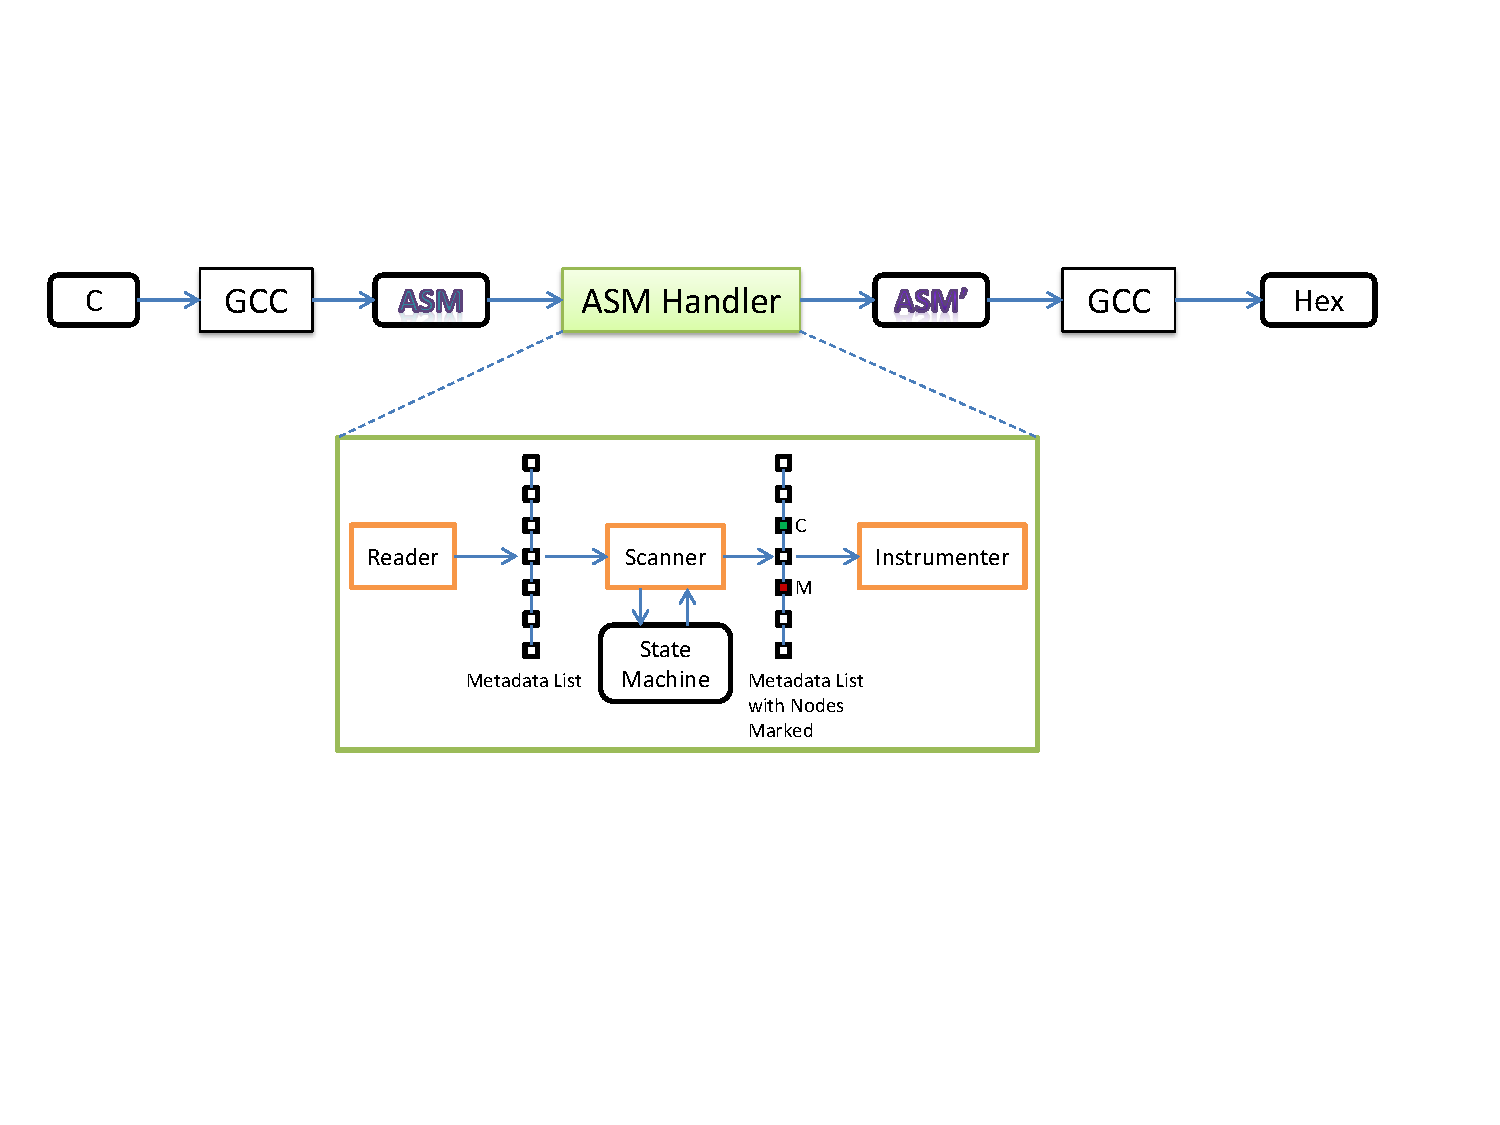
\includegraphics[width=1\textwidth]{figures/code_inject_process_v3}
%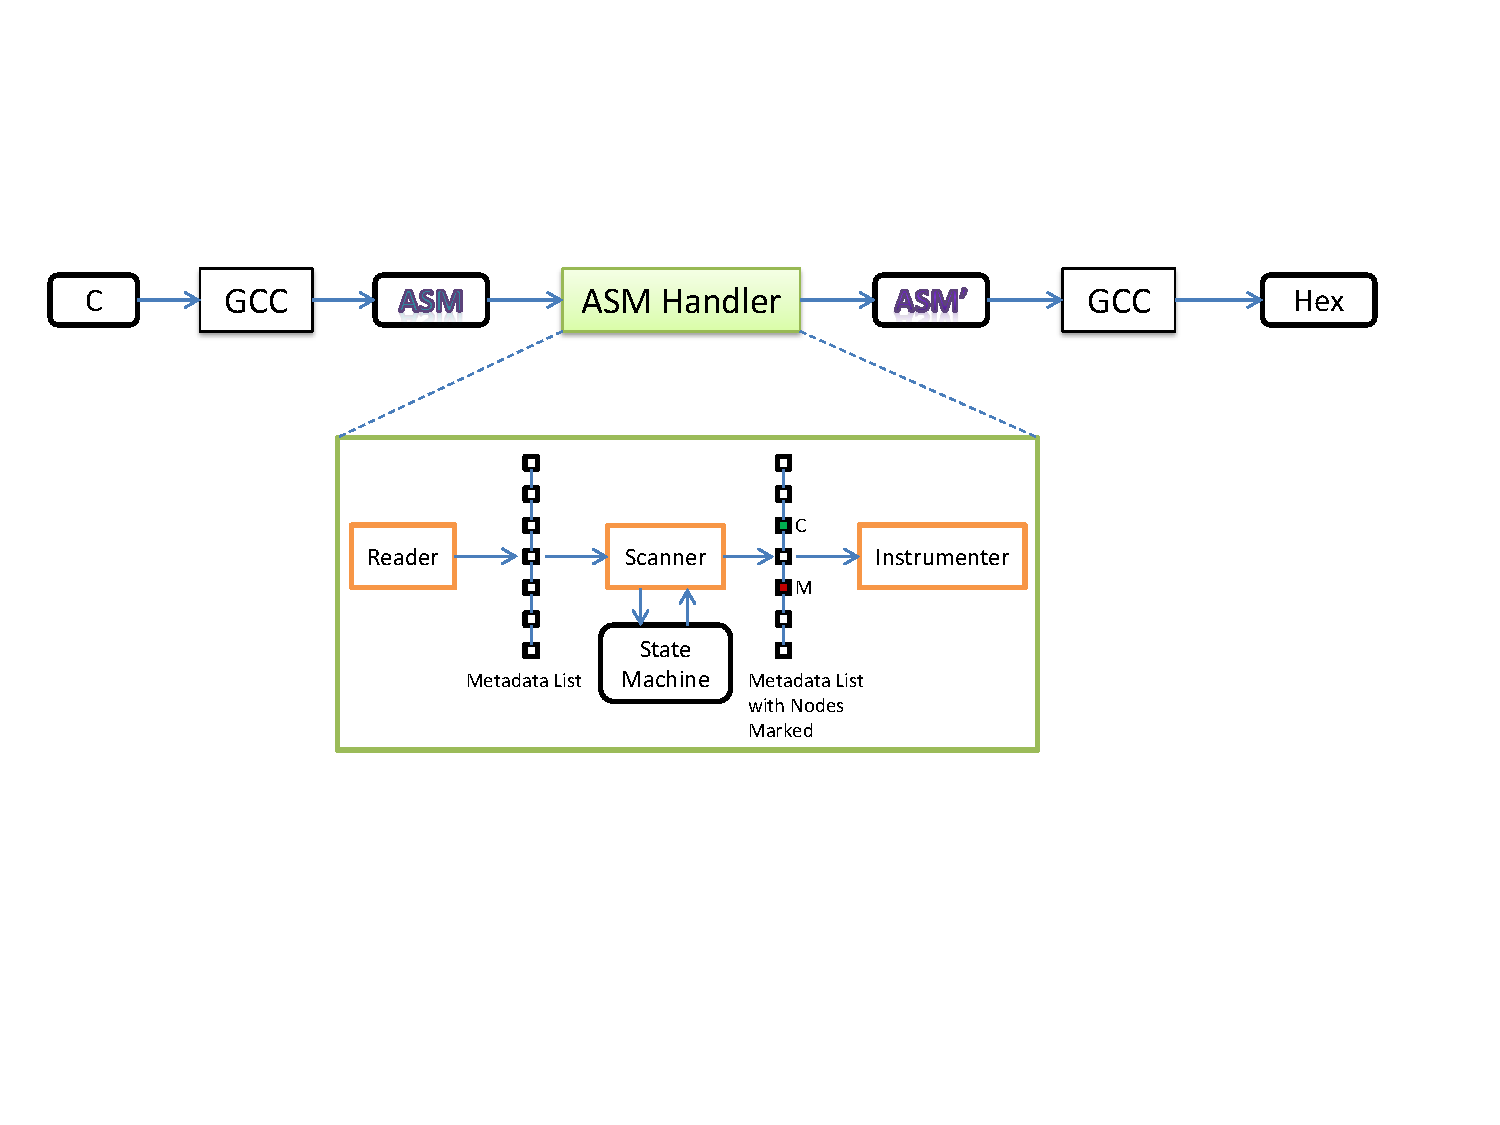
\includegraphics[width=\columnwidth]{figures/code_inject_process_v3}
\caption{Code injection Process}
\label{fig:code_injection_process}
\end{figure*}

\subsection{The ASM Handler}

The ASM Handler handles the code injection. It is designed to consist of three loose coupled modules: the \texttt{Reader}, the \texttt{Scanner}, and the \texttt{Injecter}, shown in Figure \ref{fig:code_injection_process}. A metadata is created to assist the code categorization and injection. Below is a description of the metadata and each module of the ASM Handler.

\subsubsection{ASM Metadata}

Each line of assembly code is associated with a metadata, which represents this line of code. The metadata categorizes the code into 3 categories, shown in Listing \ref{lst:metadata_example}. A \texttt{directive} is used to specify assembly code information, such as system architecture (line 1) and section (line 2), define label (line 3) ,label type (line 4), etc. A \texttt{label} is used to identify a location in the assembly code (line 5). In this example, label \texttt{main} specifies a location where the main function starts. A \texttt{instruction} is used to identify a instruction that will be executed by the microprocessor (line 6-8). The metadata also stores the code inject information, which specifies whether code is injected after this line, and the type of code to be injected.

\begin{lstlisting}[float=tb,label=lst:metadata_example,caption=Assembly Code Example]
.arch atmega644					% directive
	.text								% directive
.global	main						% directive
	.type	main, @function		% directive
main:									% label
	push r28							% instruction
	push r29							% instruction
	...
\end{lstlisting}

\subsubsection{Reader}

The Reader is used to read the assembly code file and generate a metadata list. It reads each line of the assembly code and generates a metadata node based on the assembly code. The metadata node is then appended to the metadata list. For example, the Reader generates a list with 7 nodes after it reads the assembly code in Listing \ref{lst:metadata_example}, shown in Figure \ref{fig:code_inject_process}.

\subsubsection{Scanner}

The Scanner is used to scan the metadata list, and mark the metadata nodes based on specified operations performed by the corresponding code. The marked metadata node indicates that code segments will be injected either before or after the corresponding line of code.

Since function calls follow the same process, by analyzing the execution sequence and the assembly code with the optimization level set to \texttt{none}, we identify the key operations where code segments should be injected. Below is a list of the key operations.

\begin{itemize}
\item The \texttt{Stack Frame Establishing} operation is used to 
\item The \texttt{Stack Frame Pointer Saving} operation is used to 
\item The \texttt{Function Return} operation is used to 
\end{itemize}

The Scanner scans each node in the metadata list, checks if the code represented by the node performs one of the key operations, and marks each node with a parameter set $\left\{S_{1}, S_{2}, ... S_{n}, P\right\}$, where $S_{1}$ -- $S_{n}$ are the IDs of the code segments to be injected and $P$ indicates the position of the injection (after or before the code). The node where no code will be injected is marked with an empty parameter set, $\left\{, \right\}$. For example, the metadata node that represents the xxx operation is marked with the parameter set xxx, indicating code segments xx, xx and xx to be injected before/after the represented line of code.
%The Scanner is used to scan the metadata list. Each metadata node is scanned and passed to the state machine by the Scanner. Based on the current state of the state machine after the metadata node is passed, the scanner either processes the next node, or marks the current node with parameters, indicating if code will be injected before or after the node, and what code will be injected.  For example, in Figure \ref{fig:code_inject_process}, two nodes are marked with parameters \texttt{C, B} and \texttt{M, A}, which respectively indicate CRC calculation and memory duplication code will be injected before and after corresponding nodes.

The Scanner also extracts two parameters from the metadata list. i) The Scanner detects if the \texttt{malloc} instruction is called in the target program, indicating whether the \texttt{heap} section in RAM is used, and determining the RAM section size used to store the stack frame duplicates, discussed in Section \ref{sec:memory_sections}. ii) The Scanner extracts the size of each function's stack frame by scanning the assembly code used to establish the stack frame, ``\texttt{sbiw r28, n}'', yielding a stack frame of size $n + 6$. The \texttt{n} bytes are used to store the arguments and local variables, and the additional $6$ bytes are used to store the return address, CRC, and the stack frame size, each of which takes 2 bytes.
%For each function's assembly code scanned, the Scanner also extracts two parameters. i) \texttt{Use\_Heap}, which is a boolean, is obtained by scanning if the \texttt{malloc} instruction is used in the target code. It indicates whether the \texttt{heap} section in RAM is used, determining the RAM section size used to store the stack frame duplicates, discussed in Section \ref{sec:memory_sections}. ii) \texttt{Stack\_Frame\_Size} is obtained by scanning the assembly code used to establish the stack frame, ``\texttt{sbiw r28, n}'', yielding a stack frame of size $n + 6$. The \texttt{n} bytes are used to store the arguments and local variables, and the additional $6$ bytes are used to store the return address, CRC, and the stack frame size, each of which takes 2 bytes.

\subsubsection{Injecter}

The Injecter is used to inject code segments into the target assembly code. It scans the metadata list again. When a node marked with non-empty parameter set is scanned, the Injecter injects the code segments specified in the parameter set in the position (before or after the corresponding code) specified by parameter $P$ in the parameter set. Finally, a modified assembly code file is generated, which will be assembled and linked to an executable file.


\subsection{Modified Function Execution Process}

Additional operations are added to the original function execution process by the injected code sections, performing CRC calculation, memory duplication, and other supporting operations such as register saving and restoring. Since the code sections are injected into the beginning and end of a function, the modified function execution process can be categorized into two categories, \texttt{Modified Function Invocation Process} and \texttt{Modified Function Return Process}. Below is a description of the modified function execution process.

\subsubsection{Modified Function Invocation Process}

The code segments injected into the beginning of a function is used to calculate CRC and save the duplicate of a given memory region, shown in Figure \ref{fig:modified_function_operation_pre_execution}. Figure \ref{fig:modified_function_operation_process_pre_execution} shows the execution process of the Pre-Execution Code; Figure \ref{fig:modified_function_operation_stack_pre_execution} shows the stack changes based on the Pre-Execution Code. In the execution process diagram, the white ovals show the operations performed by the original code, and the shaded ovals show the operations performed by the injected code. Each operation is labeled with a number. In the stack change diagram, \texttt{SP} is the stack pointer, and \texttt{Y} is the stack frame pointer. The numbers below each stack show the operations that changed the stack.

When function \texttt{B} is called by function \texttt{A}, the return address is pushed into the stack automatically by the function call instruction (step 1). To calculate CRC, multiple registers are used, so they must be saved before the CRC calculation process and restored when the process is finished. To avoid the calculated CRC saved in the registers being overwritten when the registers are restored, two bytes (zeros) are pushed into the stack as a placeholder (step 2) for the CRC result before the registers used to calculate CRC is saved (step 3). After the CRC of function \texttt{A}'s stack frame is calculated (step 4), the CRC result is saved to the placeholder location (step 5). The registers used to calculate CRC are then restored (step 6).

Next, the stack frame of the caller, function \texttt{A}, has to be saved. The registers used to save the stack frame are pushed into the stack (step 7). Then, the correct STP is selected by comparing the values of the three STP duplicates (step 8). Using the correct STP, the specified memory is then copied and saved in SFS (step 9). After the three STP duplicates are updated (step 10), the registers used are restored (step 11).

After the stack frame pointer of function \texttt{B} is saved (step 12) and the stack frame is established (step 13), the stack frame size of the callee, function \texttt{B}, is pushed into the stack (step 15), which is a key operation in the injected code. 

When a function is called, the return address is pushed into the stack which is used when the function returns. However, the callee function does not have context information about its caller, including the caller's stack frame address and size. It is thus impossible for the callee to calculate the CRC of the caller's stack frame and duplicate the stack frame without the information of the caller's stack frame size. To solve this problem, each function saves its stack frame size in the stack, which is used by its callee to perform CRC calculation and stack frame duplication.

\begin{figure}
        \centering
        \begin{subfigure}[b]{0.5\columnwidth}
                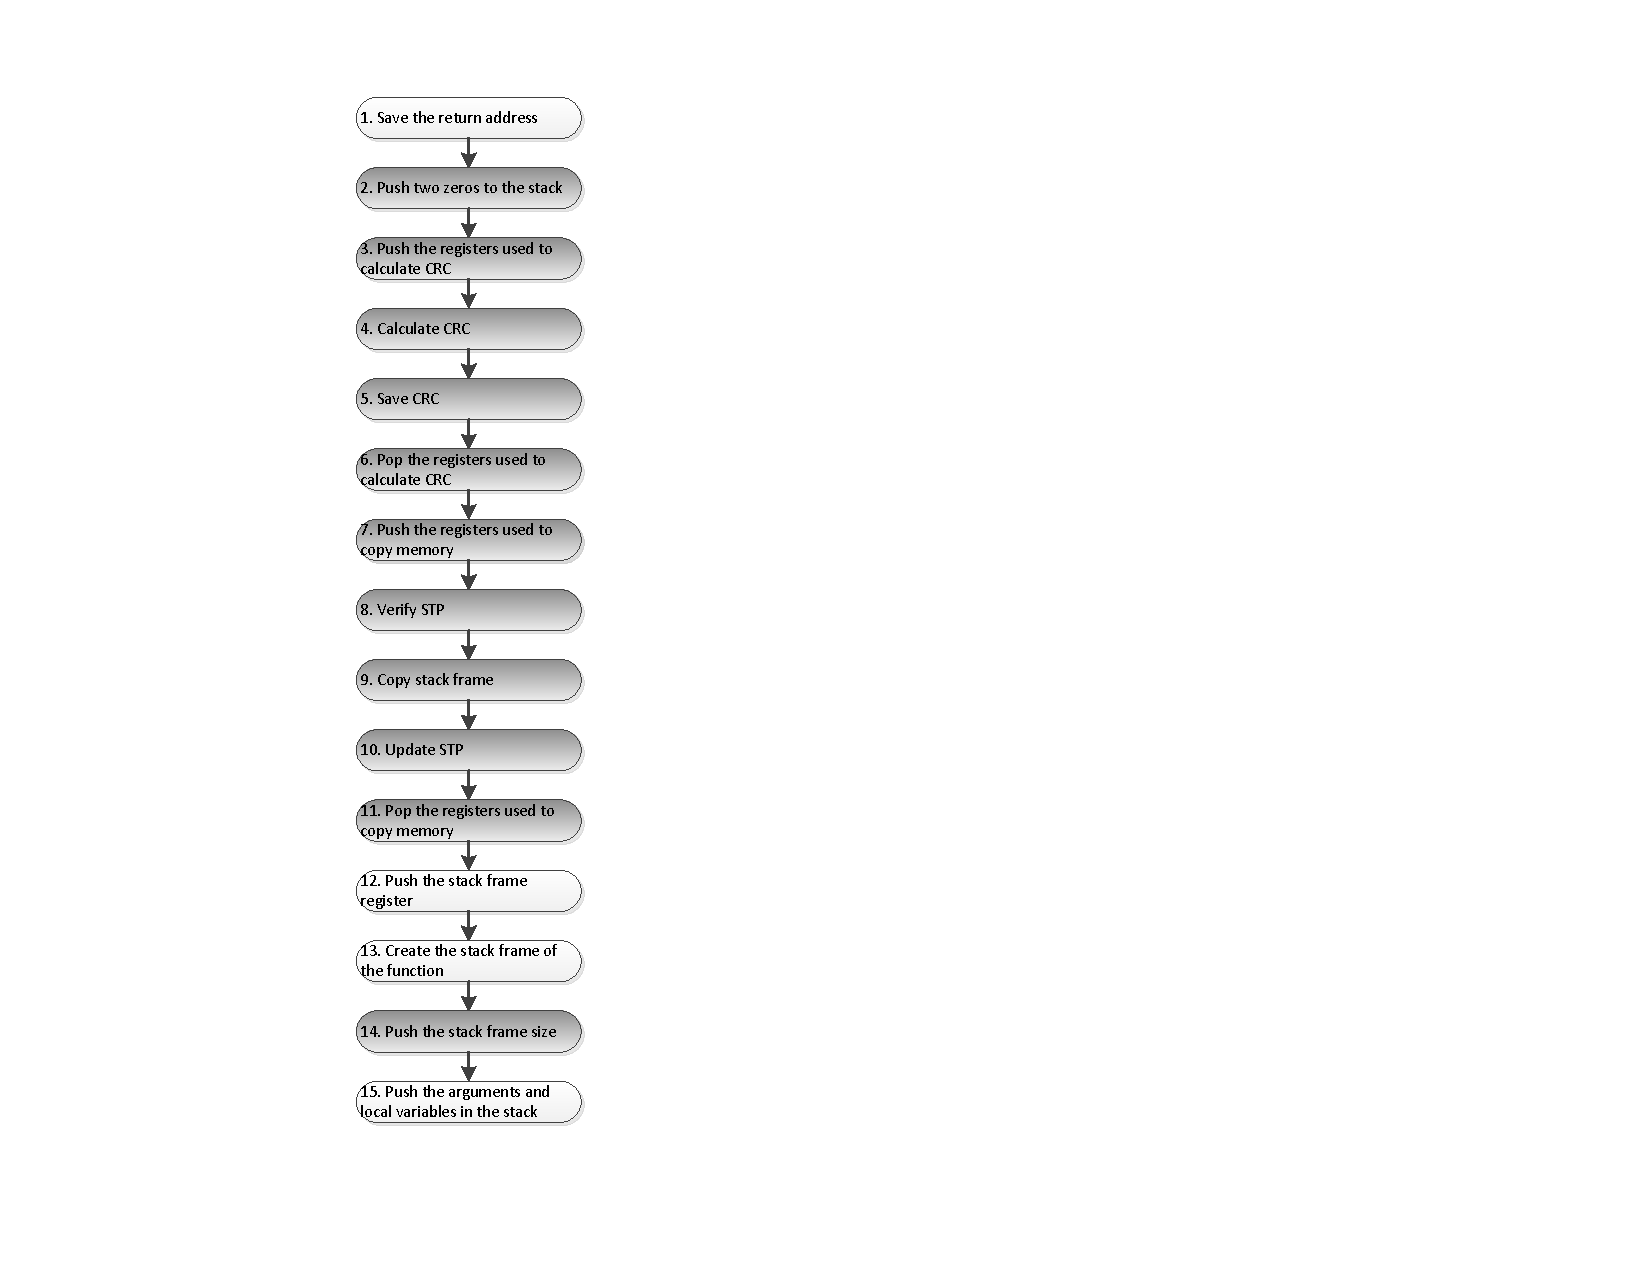
\includegraphics[width=\textwidth, height=12cm]{figures/modified_function_operations_process_pre_execution_v2}
                \caption{Process}
                \label{fig:modified_function_operation_process_pre_execution}
        \end{subfigure}~
        \begin{subfigure}[b]{0.5\columnwidth}
                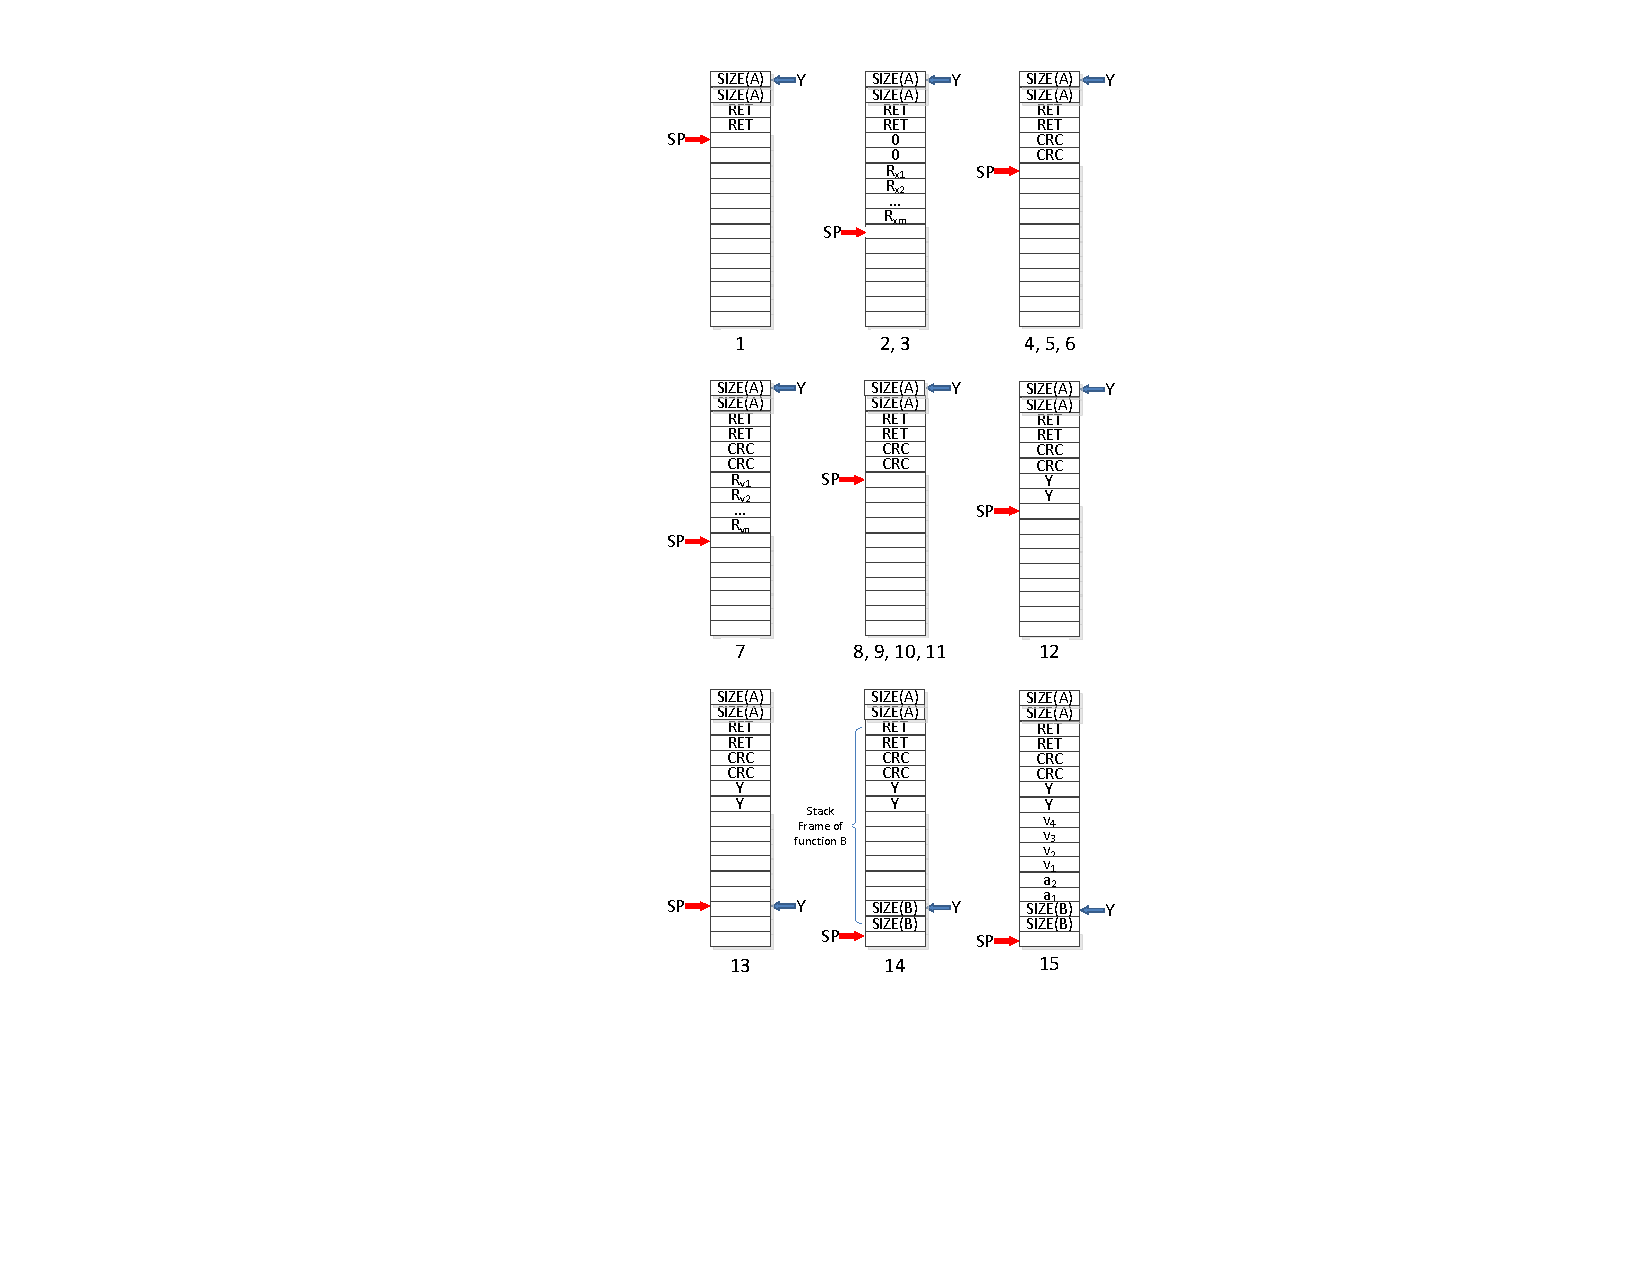
\includegraphics[width=\textwidth, height=12cm]{figures/modified_function_operations_stack_pre_execution_v1}
                \caption{Stack}
                \label{fig:modified_function_operation_stack_pre_execution}
        \end{subfigure}
        \caption{Modified Function Invocation Process}\label{fig:modified_function_operation_pre_execution}
\end{figure}

\subsubsection{Modified Function Return Process}

The code segments injected into the end of a function is used to verify the stack frame of the caller function and restore the stack frame is an SEU is detected, shown in Figure \ref{fig:modified_function_operation_post_execution}. Figure \ref{fig:modified_function_operation_process_post_execution} shows the execution process of the Post-Execution Code; Figure \ref{fig:modified_function_operation_stack_post_execution} shows the system stack changes based on the Post-Execution Code. Again, in the execution process diagram, the white ovals show the operations performed by the original code, and the shaded ovals show the operations performed by the injected code. Each operation is labeled with a number. In the stack change diagram, \texttt{SP} is the stack pointer, and \texttt{Y} is the stack frame pointer. The numbers below each stack show the operations that changed the stack.

When function \texttt{B} returns, it first pops out its stack frame size from the stack (step 1). After the space used to store the arguments and local variables is released (step 2), the stack frame pointer is restored (step 3). The CRC of function \texttt{A}'s stack frame is then calculated and temporarily stored in two registers (step 4-6). Next, the calculated CRC is compared with the CRC saved in the stack (step 7). If the two CRCs do not match, the saved stack frame of \texttt{A} is restored to the stack and the STP is updated to release the space used to store the stack frame of \texttt{A} (step 8-12). Again, the stack frame size of function \texttt{A} saved in the stack is used in CRC compare and stack frame restoration. If the two CRCs match, the STP is updated (step 13-14). After the verification of \texttt{A}'s stack frame is completed, the CRC is popped out of the stack (step 15). Finally, function \texttt{B} returns, and the return address is popped automatically (step 16).


\begin{figure}
        \centering
        \begin{subfigure}[b]{0.5\columnwidth}
                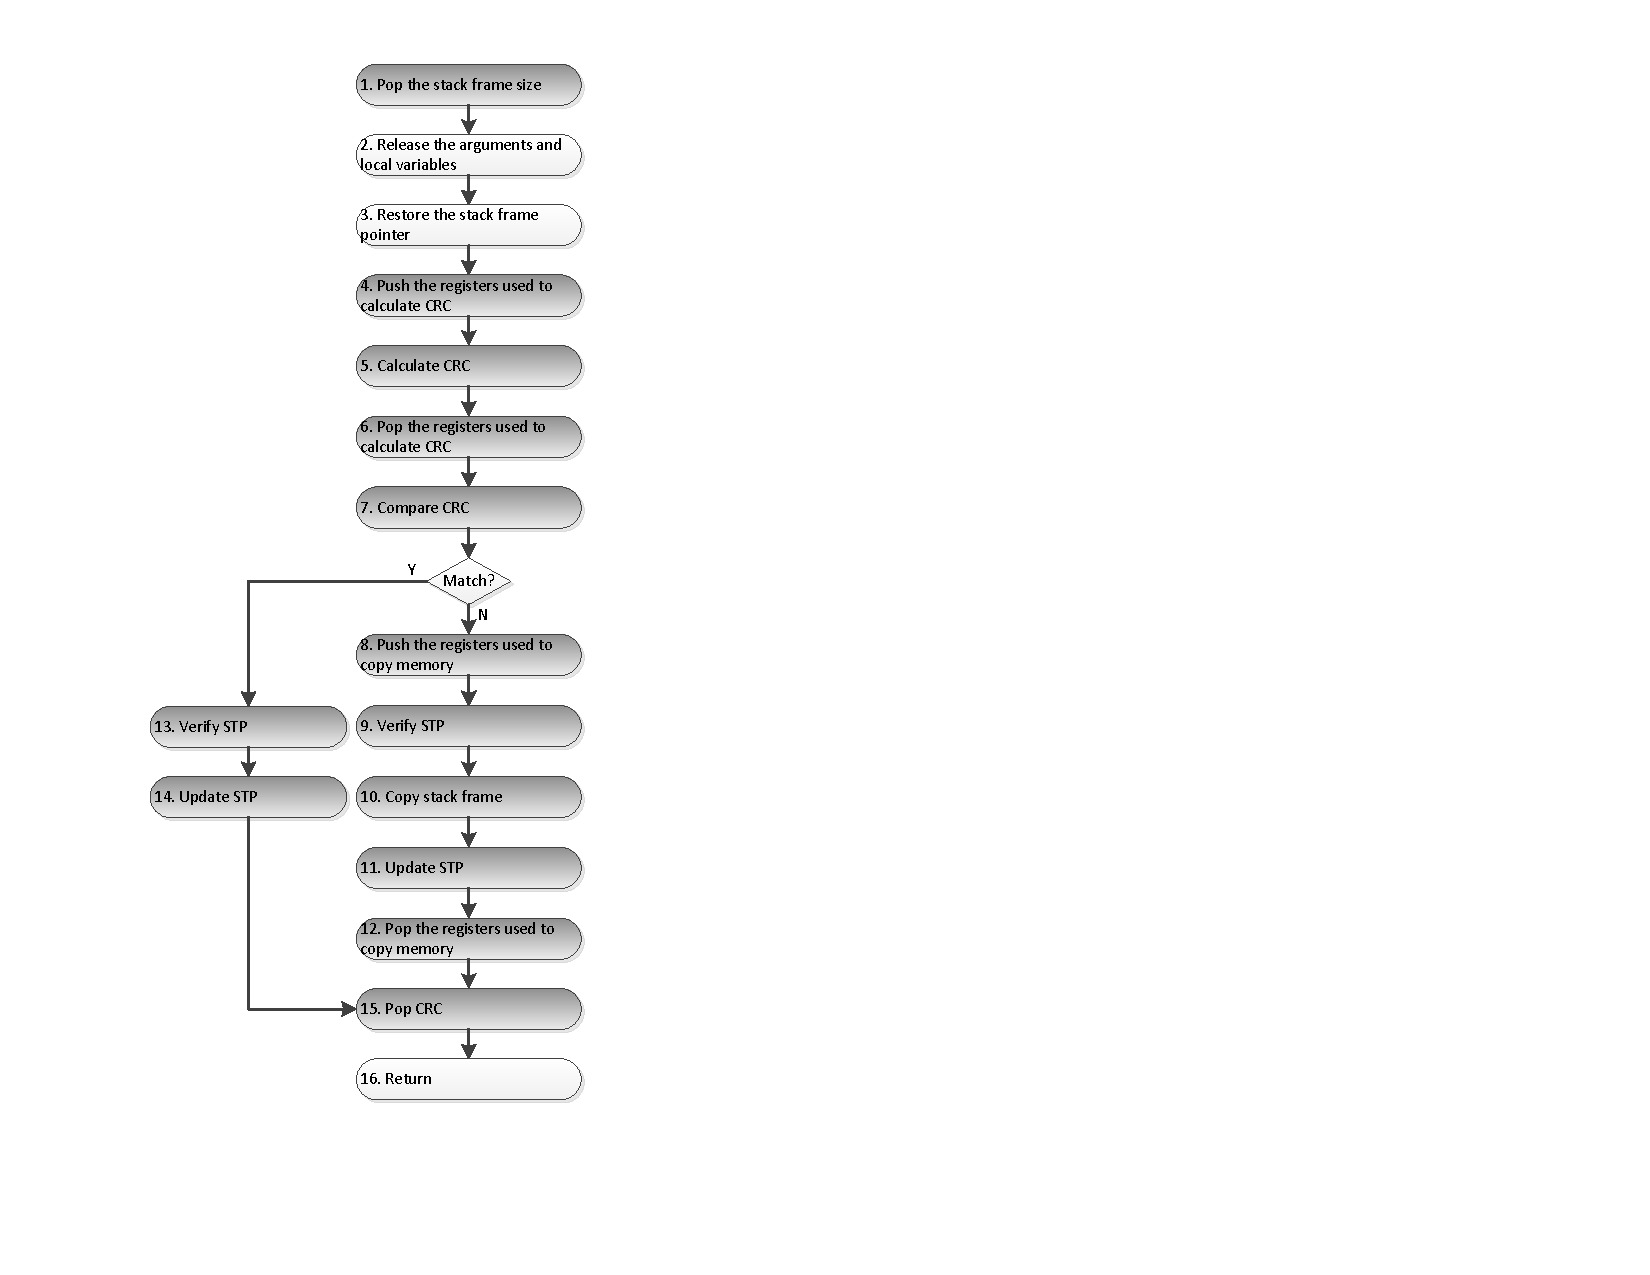
\includegraphics[width=\textwidth, height=12cm]{figures/modified_function_operations_process_post_execution_v1}
                \caption{Process Post}
                \label{fig:modified_function_operation_process_post_execution}
        \end{subfigure}~
        \begin{subfigure}[b]{0.5\columnwidth}
                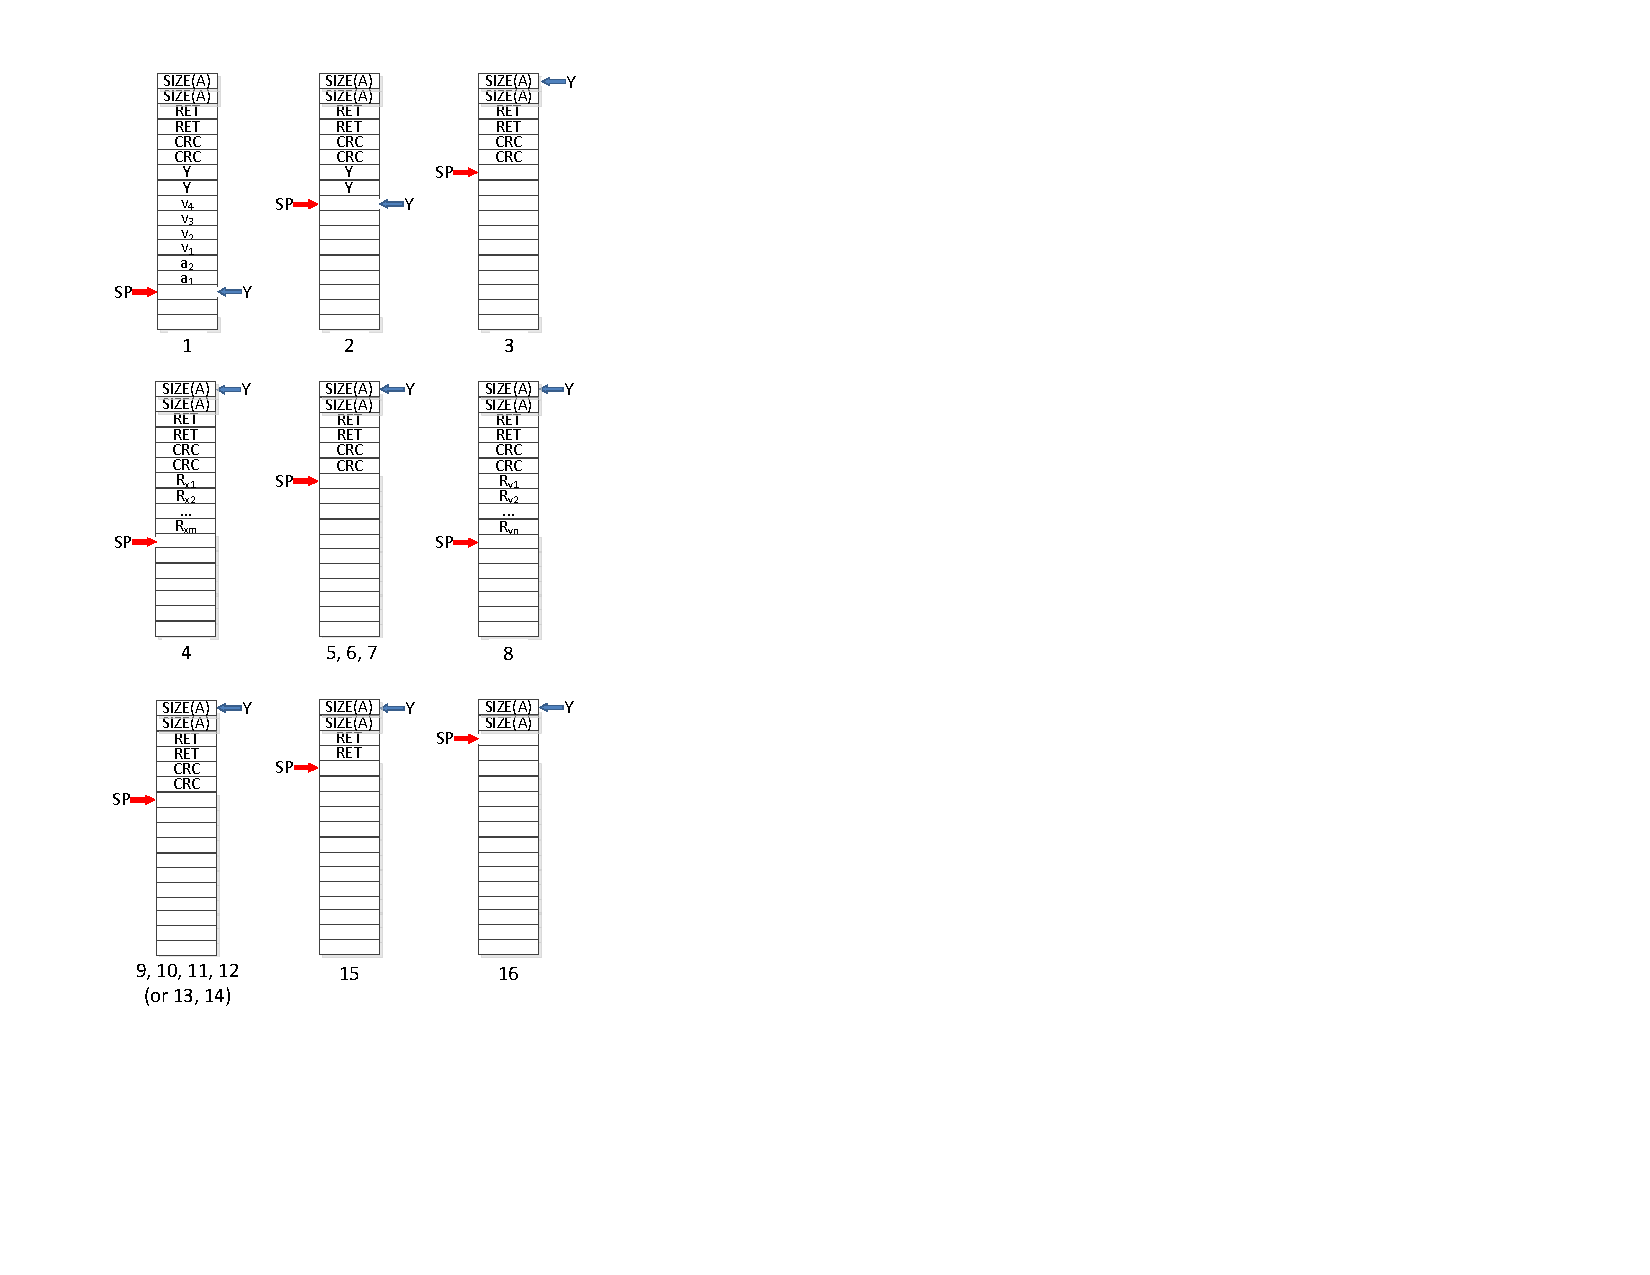
\includegraphics[width=\textwidth, height=12cm]{figures/modified_function_operations_stack_post_execution_v1}
                \caption{Stack Post}
                \label{fig:modified_function_operation_stack_post_execution}
        \end{subfigure}
        \caption{Modified Function Return Process}\label{fig:modified_function_operation_post_execution}
\end{figure}

